\documentclass[12pt]{article}
\usepackage{graphicx}
\usepackage{amsmath}
\usepackage{amsfonts}
\usepackage{enumerate}
\usepackage{amssymb}
\graphicspath{{/}}
\begin{document}
\noindent Thomas Kaunzinger\\
EECE 2540\\
Zhangyu Guan\\
10/19/2017\\
\begin{enumerate}
	\item \begin{verbatim}
from socket import *  # Import socket module
import sys            # In order to terminate the program

# Create a TCP server socket, AF_INET is used for IPv4 protocols,
# 	SOCK_STREAM is used for TCP
serverSocket = socket(AF_INET, SOCK_STREAM)

# Assign a port number
serverPort = 12000

# Bind the socket to server address and server port
serverSocket.bind(('',serverPort))

# Listen to at most 1 connection at a time
serverSocket.listen(1)

# Server should be up and running and listening to the incoming connections
while True:
    print('The server is ready to receive')

    # Set up a new connection from the client
    connectionSocket, addr = serverSocket.accept()

    # If an exception occurs during the execution of try clause,
    # 	the rest of the clause is skipped
    # If the exception type matches the word after except,
    # 	the except clause is executed
    try:
        # Receives the request message from the client
        message = connectionSocket.recv(1024).decode()

        messageSplit = message.split()

        # Extract the path of the requested object from the message
        # The path is the second part of HTTP header, identified by [1]
        filepath = messageSplit[1]

        # Because the extracted path of the HTTP request includes 
        # a character '\', we read the path from the second character 
        filepathName = filepath[1:]

        # Store the entire contenet of the requested file in
        # 	a temporary buffer
        fileBuffer = open(filepathName)
        fileString = fileBuffer.read()


        # Send the HTTP response header line to the connection socket
        connectionSocket.send(("HTTP/1.1 200 OK\n"
                                + "Content-Type: text/html\n"
                                + "\n").encode())

        # Send the content of the requested file to the connection socket
        connectionSocket.send(fileString.encode())

        # Close the client connection socket
        connectionSocket.close()

        # Closes the server socket after a request is processed
        serverSocket.close()

        #Terminate the program after sending the corresponding data
        sys.exit()

	except IOError:
        # Opens and reads custom 404 page HTML file
        fof = open("fof.html")
        fofRead = fof.read()

        # Sends HTTP response message and page for file not found
        connectionSocket.send(("HTTP/1.1 404 Not Found\n"
                                + "Content-Type: text/html\n"
                                + "\n").encode())
        connectionSocket.send(fofRead.encode())

        # Close the client connection socket
        connectionSocket.close()

        # Closes the server socket after a request is processed
        serverSocket.close()

        #Terminate the program after sending the corresponding data
        sys.exit()
		
		\end{verbatim}

		Two test files (HTML files made back in highschool) and a 404 page all grabbed from the local server using the local address (127.0.0.1) on port 12000.\\
		\\
		Example URL: http://127.0.0.1:12000/kyle.html\\
		\\
		Test 1: Request kyle.html\\
		\\
		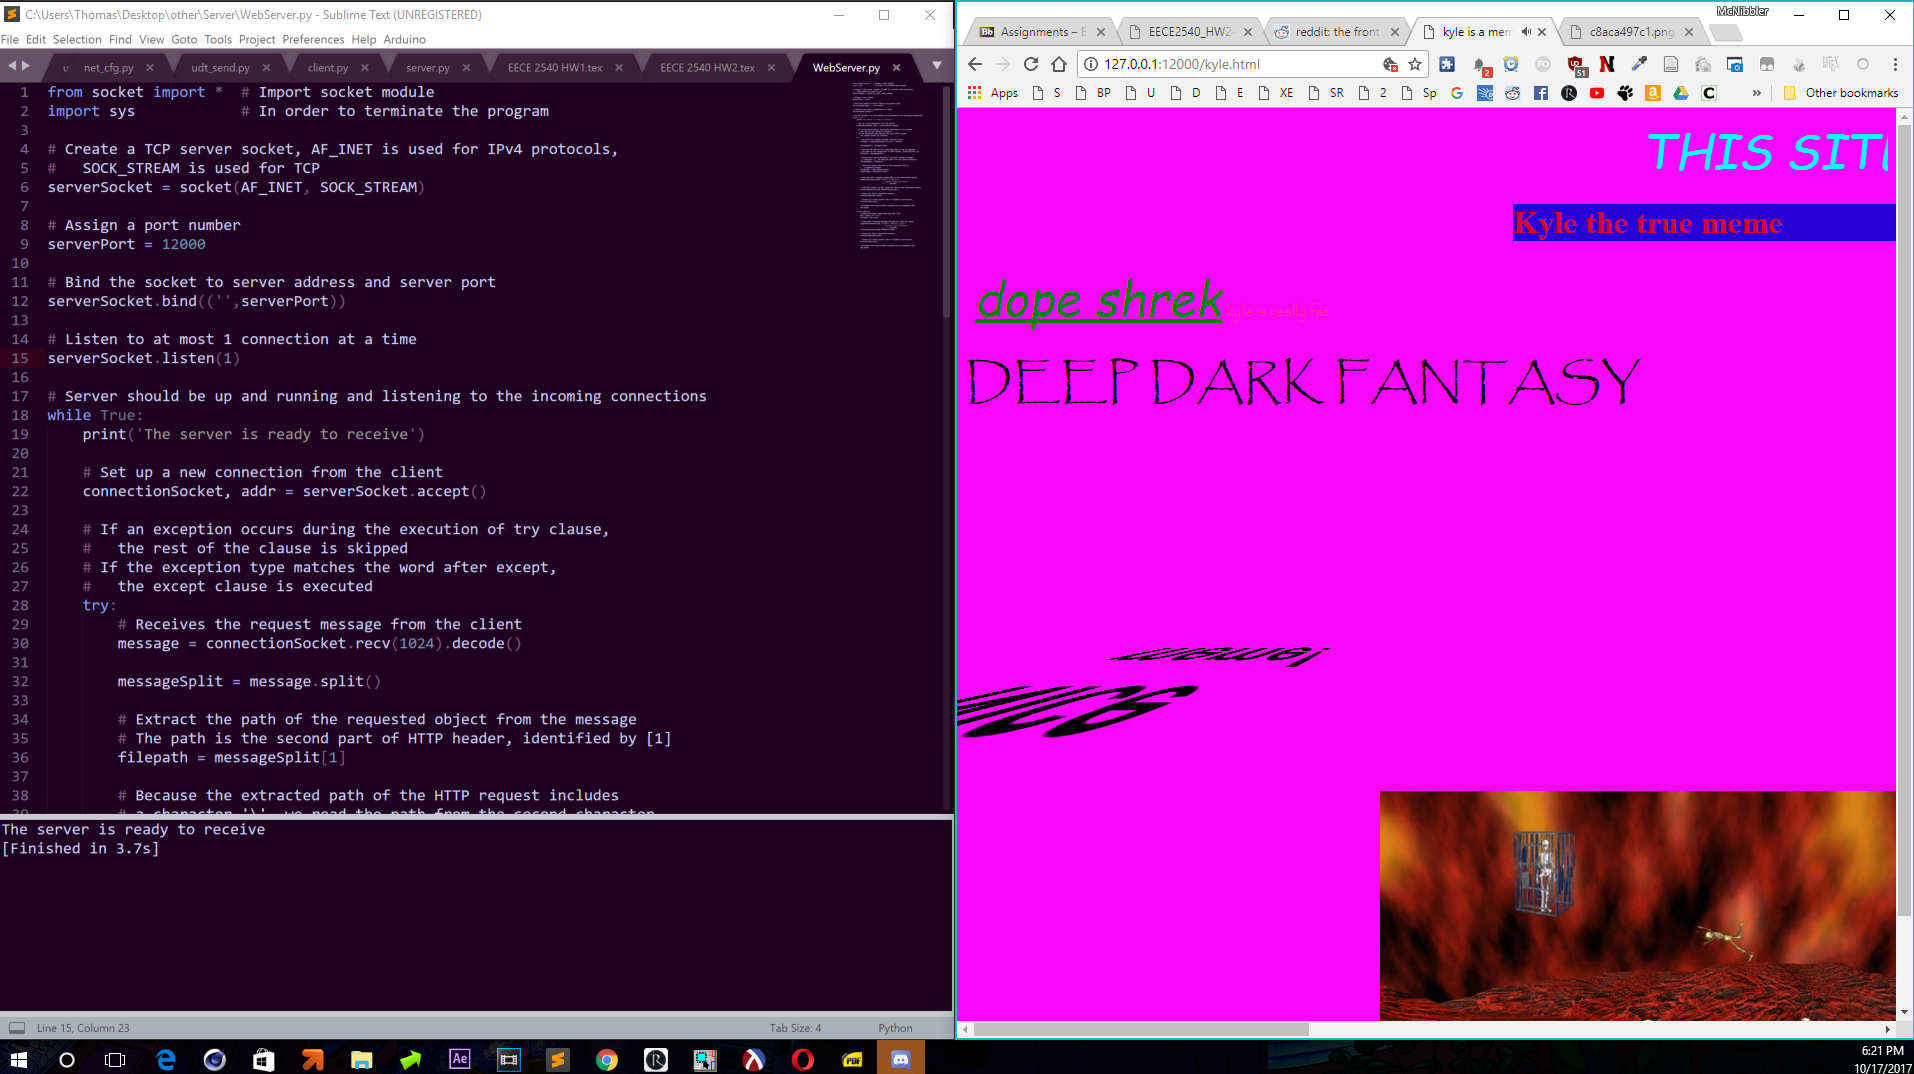
\includegraphics[scale=0.4]{TestHTML1}\\
		\\
		\\
		\\
		\\
		Test 2: Request shrex.html\\
		\\
		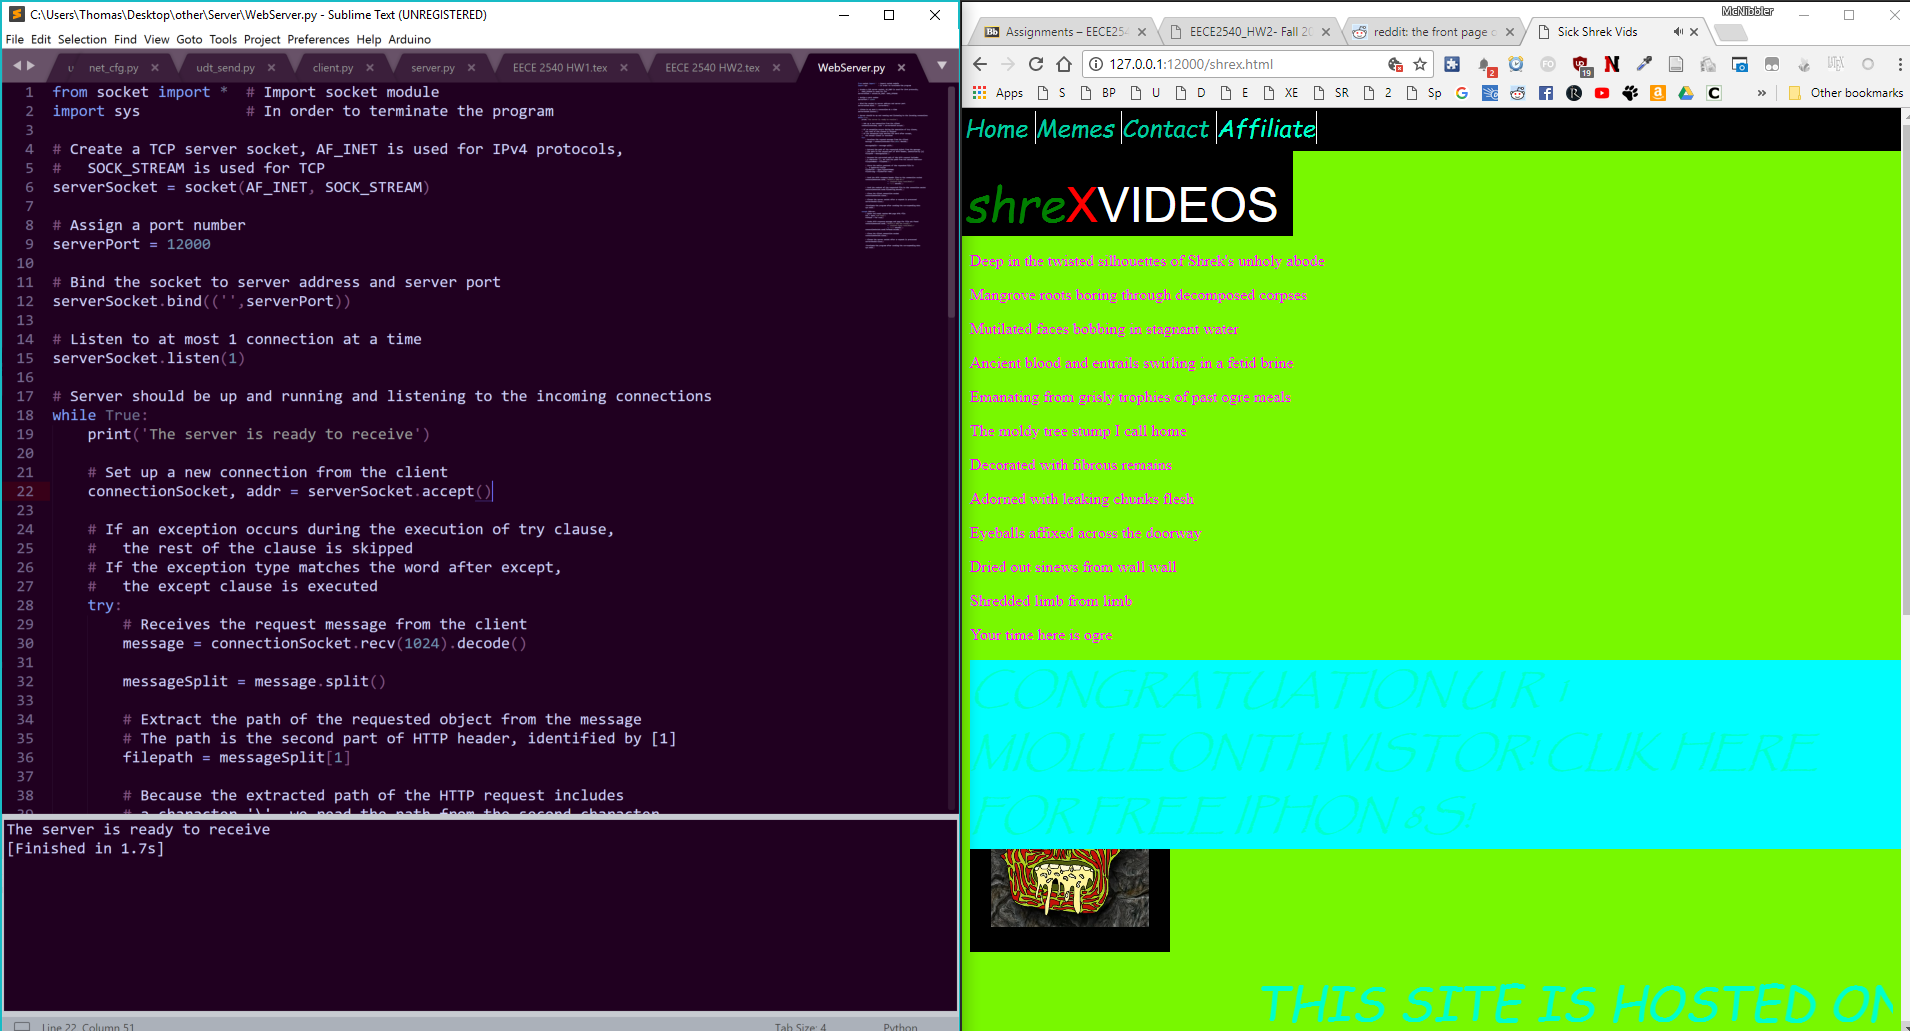
\includegraphics[scale=0.4]{TestHTML2}\\
		\\
		\\
		Test 3: Request thisfiledoesntexist.txt\\
		Recieved fof.html (failsafe 404 page)\\
		\\
		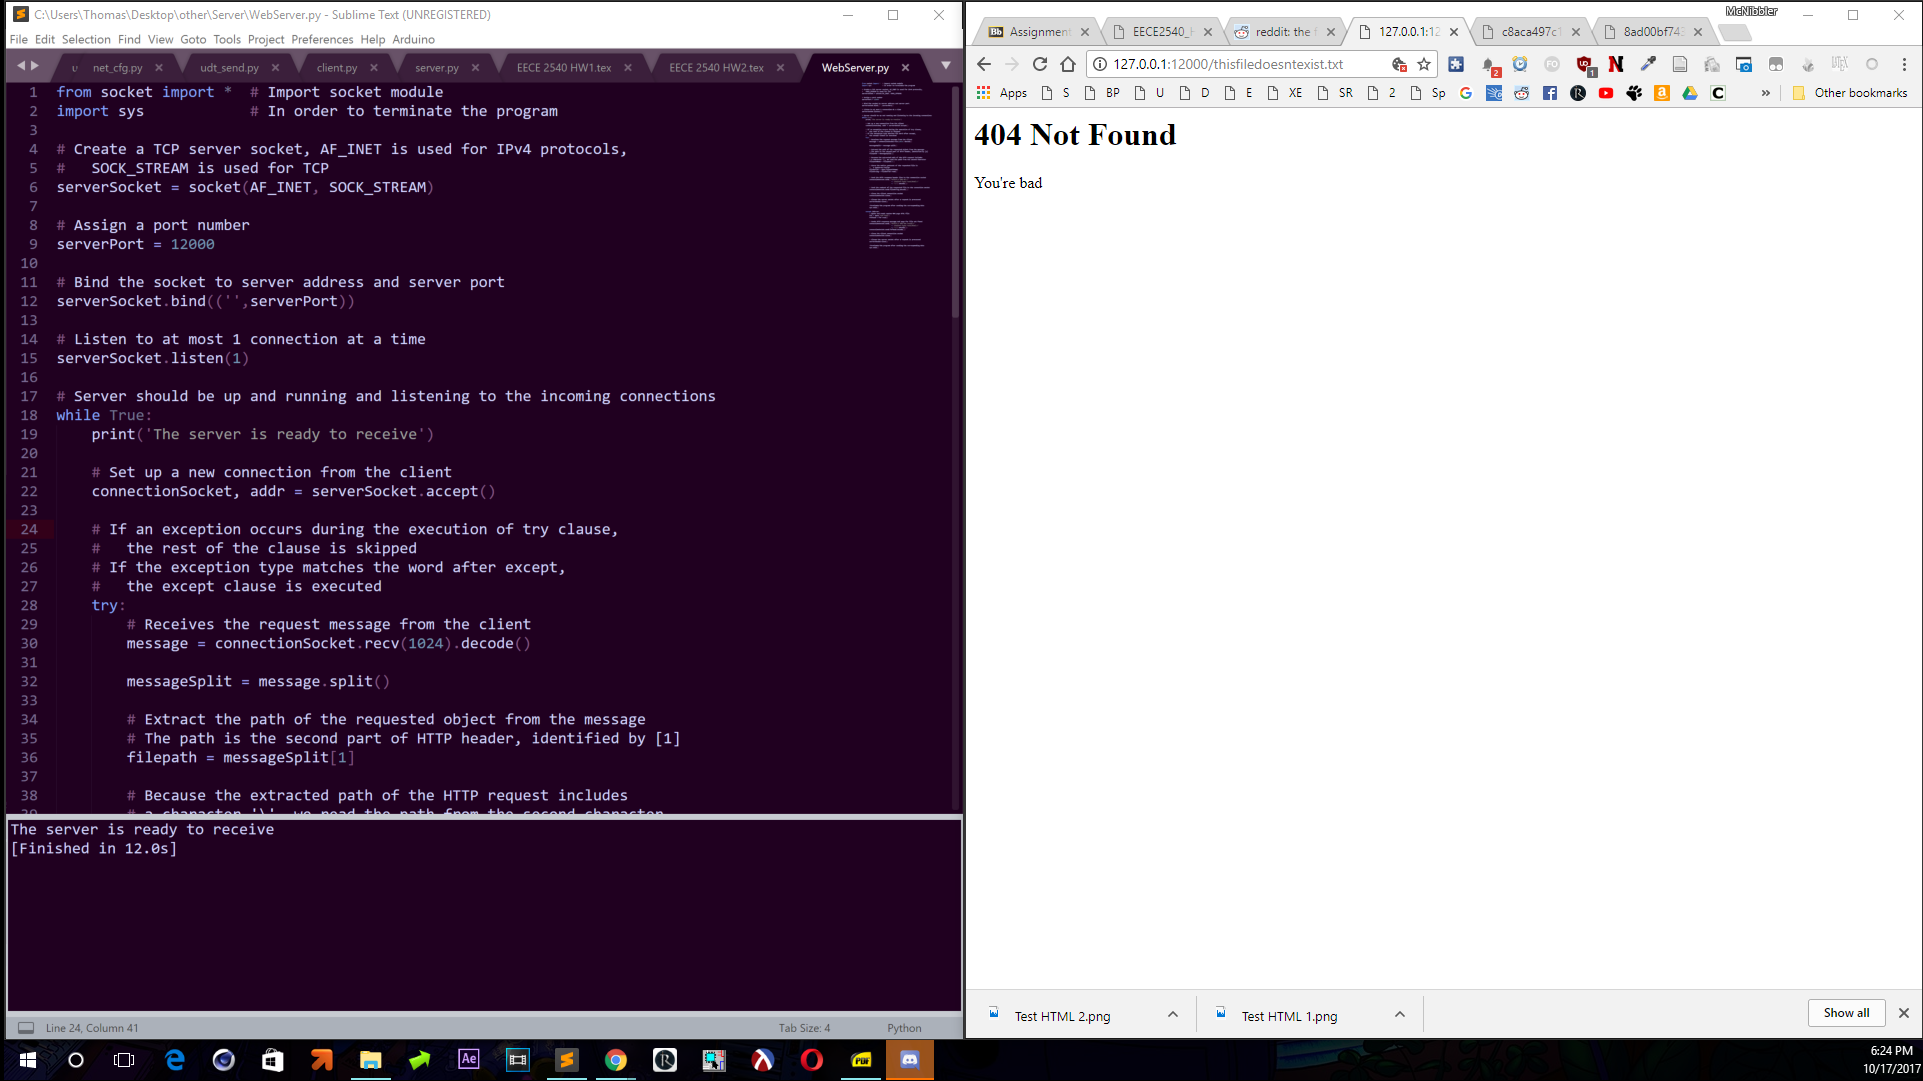
\includegraphics[scale=0.4]{Test404}\\

	\item \begin{enumerate}
			\item An application using UDP does not need to establish a connection and communicate with each individual user to ensure each packet is sent correctly. This is useful in a situation where it is unimportant wether or not a user recieves every packet, such as in a live video feed. Since the protocol is simpler, more data can be sent per packet and there is no response delay.
			\\
			\item With TCP, a short buffer (resulting in slight video delay) can be used to ensure that the sender is recieving all packets correctly in the right order so that the sender is not sending packets that persistently get dropped (such as a with a very high bitrate that overwhelms the reciever).
			\item UDP can still be reliable but only at the application layer, as the application will have to have its own methods of error recovery, such as with a UDP checksum, which checks if a single bit has flipped in small chunks, and then send NAKs when packets are incorrect.
			\item Since UDP is a connectionless protocol, the sender doesnt have to recieve any responses from the reciever. Multiple sources can send packets on the same port and the reciever will recieve packets in order of them being recieved with headers that show where each packet was sent from.
			\item Sequence numbers are added to show which packets have been recieved and prevent duplicate packets. If a sender recieves an ACK with a sequence number, it knows which packets the reciever has gotten and if it has dropped any and will send packets further along the sequence number before getting another response telling which sequence of packets to start from.
			\item If the reciever does not send back an ACK, the sender will retransmit within a reasonable amount of time, as either the packet was lost getting to the reciever, or the ACK was lost, to which the sequence number will be able to determine which of the retransmitted packets are duplicates.
		\end{enumerate}

	\item Since the sender is only sending data infrequently, it would make more sense for the reciever to immediately acknowledge that it got its small packet of data correctly instead of persistently saying when it doesn't recieve it, to which the only indication that it does recieve it is when it does not say it did not recieve a packet very infrequently. If a packet was dropped, it won't know until it gets the acknowledgement from the next packet, leading to a long error recovery time.


	Conversely, in the situation where the sender sends frequently over a fairly reliable connection, it makes more sense for the reciever to send a NAK when needed, as generally speaking it's expected that the packets are going to send correctly and it will save time to just send a response when something goes wrong instead of saying it's right every time.

	\item Using this pipelining technique with alternating bits for the ACKs could potentially allow for a much higher use of the channel as, in theory, the sender would check for ACKs and check if their bit is the opposite of that of the previous ACK. Theoretically, if the sender recieves an ACK with the same bit as the previous, it means that a packet was lost. However, since there's only two states and there are many more packets than that being sent at once, the sender will have no way of telling which packets actually correspond to which ACK recieved if it does in fact detect that there's an error, completely bypassing the security of RDT.

	\item With selective repeat, a sender can recieve an ACK outside of its current window. If the timer expires too quickly after the reciever sends its ACKs, the sender will send the window packets again and the reciever can send the duplicate ACKs. When the Sender recieves the first set of ACKs that were still sending while the timer expired, the window will change to the next set of packets, to which the sender will send the next packets only to soon recieve the duplicate ACKs from the previous window.\\
	\\
	\includegraphics[scale=0.05]{question5}\\

	\item From top to bottom X
		\begin{enumerate}
			\item Host A is sending 120 bytes including the starting sequence number 50 (49 bytes already have been exchanged).\\
			\\
			$byte = 49 + 120$\\
			\\
			$byte = 169$\\
			\\
			Since ACK asks for the next byte required\\
			\\
			$ACK = byte + 1 = 170$\\
			\item Host B sends $ACK 170$, which is the next byte to be requested\\
			\\
			Sequence No. = ACK No.\\
			\\
			$\text{Sequence No} = 170$\\
			\item Host B is sending 550 bytes starting on sequence 400, meaning that it has already taken care of the previous 399 bytes and will send 550 back to host A.\\
			\\
			$byte = 399 + 550$\\
			\\
			$byte = 949$\\
			\\
			Since ACK asks for the next byte required\\
			\\
			$ACK = byte + 1 = 950$\\

		\end{enumerate}

	\item $RTT = 10 \times D_{trans}$\\
			\\
			$D_{trans} = \dfrac{25670\text{ bits}}{10^{9}\text{ bps}}$\\
			\\
			$D_{trans} = 0.02567ms$\\
			\\
			$RTT = 10 \times 0.02567ms$\\
			\\
			$RTT = 0.25670ms$
		\begin{enumerate}
			\item $\text{Utilization}_{stop} = \dfrac{D_{trans}}{D_{trans} + RTT}$\\
				\\
				$\text{Utilization}_{stop} = \dfrac{0.02567ms}{0.02567ms + 0.25670ms}$\\
				\\
				$\text{Utilization}_{stop} = \dfrac{0.02567ms}{0.28237ms}$\\
				\\
				$\text{Utilization}_{stop} = 9.091\%$
			\item $\text{Utilization}_{pipe} = \text{Utilization}_{stop} \times \text{packets}$\\
				\\
				$\text{Utilization}_{pipe} = 9.091\% \times 5$\\
				\\
				$\text{Utilization}_{pipe} = 45.455\%$
		\end{enumerate}

	\item \begin{enumerate}
			\item UDP has to attatch a port and destination address to every packet because the protocol does not establish a connection beforehand between the sender and reciever, meaning that the host otherwise does not know who it is connected with but rather simply the address it gets from the requested packet.
			\item UDP does need a source address for its outgoing packets because it is connectionless and simply broadcasting to those who are requesting from a socket. Since there is no established connection between the host and client, the source address is needed so that the client has a way to communicate back to the server. The application code does this through the socket library.
			\item A socket "bind" function assigns a port number to a socket so that the socket can access data on that port, whether it be recieving or sending. Furthermore, listen is used in TCP to open the port and see if a client is sending a message to the host. The parameter specifies how many users can connect before it refuses new connections.
			\item The TCP function connect() establishes a handshake connection by contacting the server with its socket information and guarantees contact between the client and server, ensuring that sending a packet automatically sends it through the right socket. The programs are aware as if the connection isn't established properly, the program sends back an error preventing use of the socket.
		\end{enumerate}

\end{enumerate}

\end{document}